\documentclass[a4paper]{article}
\usepackage{verbatim}
\usepackage{pgf,tikz}
\usetikzlibrary{positioning, arrows.meta, matrix, backgrounds, shapes.misc}
\usetikzlibrary{calc,arrows}
\usepackage{amsmath}
\usepackage[left=1cm,right=1cm]{geometry}
\pagestyle{empty}
%\usetikzlibrary{shapes.multipart}

\makeatletter


\begin{comment}
\end{comment}

% Data Flip Flip (DFF) shape
\pgfdeclareshape{dff}{
	% The 'minimum width' and 'minimum height' keys, not the content, determine
	% the size
	\savedanchor\northeast{%
		\pgfmathsetlength\pgf@x{\pgfshapeminwidth}%
		\pgfmathsetlength\pgf@y{\pgfshapeminheight}%
		\pgf@x=0.5\pgf@x
		\pgf@y=0.5\pgf@y
	}
	% This is redundant, but makes some things easier:
	\savedanchor\southwest{%
		\pgfmathsetlength\pgf@x{\pgfshapeminwidth}%
		\pgfmathsetlength\pgf@y{\pgfshapeminheight}%
		\pgf@x=-0.5\pgf@x
		\pgf@y=-0.5\pgf@y
	}
	% Inherit from rectangle
	\inheritanchorborder[from=rectangle]
	
	% Define same anchor a normal rectangle has
	\anchor{center}{\pgfpointorigin}
	\anchor{north}{\northeast \pgf@x=0pt}
	\anchor{east}{\northeast \pgf@y=0pt}
	\anchor{south}{\southwest \pgf@x=0pt}
	\anchor{west}{\southwest \pgf@y=0pt}
	\anchor{north east}{\northeast}
	\anchor{north west}{\northeast \pgf@x=-\pgf@x}
	\anchor{south west}{\southwest}
	\anchor{south east}{\southwest \pgf@x=-\pgf@x}
	\anchor{text}{
		\pgfpointorigin
		\advance\pgf@x by -.5\wd\pgfnodeparttextbox%
		\advance\pgf@y by -.5\ht\pgfnodeparttextbox%
		\advance\pgf@y by +.5\dp\pgfnodeparttextbox%
	}
	
	% Define anchors for signal ports
	\anchor{D}{
		\pgf@process{\northeast}%
		\pgf@x=-1\pgf@x%
		\pgf@y=.5\pgf@y%
	}
	\anchor{CLK}{
		\pgf@process{\northeast}%
		\pgf@x=-1\pgf@x%
		\pgf@y=-.66666\pgf@y%
	}
	\anchor{CE}{
		\pgf@process{\northeast}%
		\pgf@x=-1\pgf@x%
		\pgf@y=-0.33333\pgf@y%
	}
	\anchor{Q}{
		\pgf@process{\northeast}%
		\pgf@y=.5\pgf@y%
	}
	\anchor{Qn}{
		\pgf@process{\northeast}%
		\pgf@y=-.5\pgf@y%
	}
	\anchor{R}{
		\pgf@process{\northeast}%
		\pgf@x=0pt%
	}
	\anchor{S}{
		\pgf@process{\northeast}%
		\pgf@x=0pt%
		\pgf@y=-\pgf@y%
	}
	% Draw the rectangle box and the port labels
	\backgroundpath{
		% Rectangle box
		\pgfpathrectanglecorners{\southwest}{\northeast}
		% Angle (>) for clock input
		\pgf@anchor@dff@CLK
		\pgf@xa=\pgf@x \pgf@ya=\pgf@y
		\pgf@xb=\pgf@x \pgf@yb=\pgf@y
		\pgf@xc=\pgf@x \pgf@yc=\pgf@y
		\pgfmathsetlength\pgf@x{1.6ex} % size depends on font size
		\advance\pgf@ya by \pgf@x
		\advance\pgf@xb by \pgf@x
		\advance\pgf@yc by -\pgf@x
		\pgfpathmoveto{\pgfpoint{\pgf@xa}{\pgf@ya}}
%		\pgfpathlineto{\pgfpoint{\pgf@xb}{\pgf@yb}}
%		\pgfpathlineto{\pgfpoint{\pgf@xc}{\pgf@yc}}
		\pgfclosepath
		
		% Draw port labels
		\begingroup
		\tikzset{flip flop/port labels} % Use font from this style
		\tikz@textfont
		\endgroup
	}
}

% Key to add font macros to the current font
\tikzset{add font/.code={\expandafter\def\expandafter\tikz@textfont\expandafter{\tikz@textfont#1}}} 

% Define default style for this node
\tikzset{flip flop/port labels/.style={font=\sffamily\scriptsize}}
\tikzset{every dff node/.style={draw,minimum width=1.0cm,minimum 
		height=0.5cm,very thick,inner sep=1mm,outer sep=0pt,cap=round,add 
		font=\sffamily}}

\makeatother

\begin{document}

	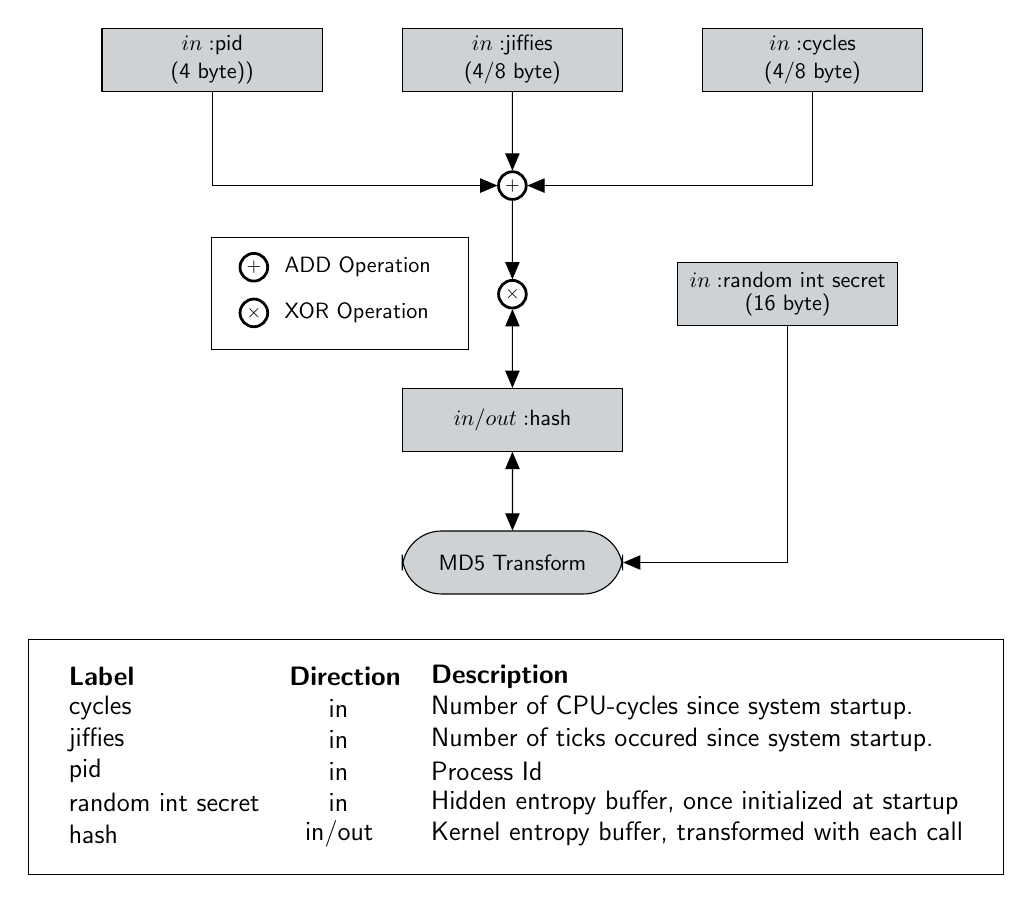
\begin{tikzpicture}[scale=0.8, every node/.style={scale=0.8},font=\sffamily,>=triangle 45]
	\tikzstyle{sum} = [draw, shape=circle, node distance=1.5cm, line width=1pt, minimum width=1.25em]	
	%\Huge
	\def\N{7}  % Number of Flip-Flops minus one
	\def\BW{1.8} % Byte Width
	
	% colors
	\definecolor{cjh}{HTML}{CFD2D4}
	\definecolor{cjl}{HTML}{DD6262}
	\definecolor{cch}{HTML}{F7A100}
	\definecolor{ccl}{HTML}{0288CF}
	\definecolor{cep32}{HTML}{64FE2E}
	\definecolor{cep1}{HTML}{1893D4}
	\definecolor{cep0}{HTML}{A9FD2A}
	\definecolor{cirq}{HTML}{DB15E5}
	\definecolor{cip}{HTML}{FFF200}
	
	% rect rc-inp-pid
	\node (rc-inp-pid) [rectangle, fill=cjh, draw, minimum width=35mm, minimum height=10mm, anchor= south west] at (0,0) {\shortstack{$in:$pid\\(4 byte))}};
	% rect rc-inp-jiffies
	\node (rc-inp-jiffies) [rectangle, right=10mm of rc-inp-pid, fill=cjh, draw, minimum width=35mm, minimum height=10mm, anchor= west] {\shortstack{$in:$jiffies\\(4/8 byte)}};	
	% rect rc-inp-cycles	
	\node (rc-inp-cycles) [rectangle, right=10mm of rc-inp-jiffies, fill=cjh, draw, minimum width=35mm, minimum height=10mm, anchor= west] {\shortstack{$in:$cycles\\(4/8 byte)}};	
	% oa-pjc - add pid/jiffies/cycles
	\node [sum, below=10mm of rc-inp-jiffies, draw] (oa-pjc) {};	
	\node at (oa-pjc) (plus) {{\footnotesize$+$}};	
	% rc-inp-pid -> oa-pjc
	\draw [->] (rc-inp-pid) |- (oa-pjc);	
	% rc-inp-jiffies -> oa-pjc
	\draw [->] (rc-inp-jiffies) -- (oa-pjc);
	% rc-inp-cycles -> oa-pjc
	\draw [->] (rc-inp-cycles) |- (oa-pjc);
	% ox-oa-pjc-hash 
	\node [sum, below=10mm of oa-pjc, draw] (ox-oa-pjc-hash) {};	
	\node [rotate=45] at (ox-oa-pjc-hash) (plus) {{\footnotesize$+$}};	
	% oa-pjc -> ox-oa-pjc-hash
	\draw [->] (oa-pjc) -- (ox-oa-pjc-hash);	
	% rc-hash	
	\node (rc-hash) [rectangle, below=10mm of ox-oa-pjc-hash, fill=cjh, draw, minimum width=35mm, minimum height=10mm] {\shortstack{$in/out:$hash}};		
	% ox-oa-pjc-hash <-> md5-transf
	\draw [<->] (ox-oa-pjc-hash) -- (rc-hash);	
	% md5-transf
	\node (md5-transf) [rectangle, below=10mm of rc-hash, fill=cjh, draw, minimum width=35mm, minimum height=10mm, rounded corners=0.5cm] {\shortstack{MD5 Transform}};	
	% rc-hash <-> md5-transf
	\draw [<->] (rc-hash) -- (md5-transf);
	% rect rc-rnd-int-sec
	\node (rc-rnd-int-sec) [rectangle, right=19mm of ox-oa-pjc-hash, fill=cjh, draw, minimum width=35mm, minimum height=10mm, anchor= west] {\shortstack{$in:$random int secret\\(16 byte)}};	
	% rc-rnd-int-sec <-> md5-transf
	\draw [->] (rc-rnd-int-sec) |- (md5-transf);
	
	%%%%%%%%% Legende
	\begin{scope}
	
	% ox
	\node [sum,  below right=25mm and 18mm of rc-inp-pid.west, draw] (loa) {};	
	\node at (loa) (plus) {{\footnotesize$+$}};	
	\node[black, right=1mm of loa.east, anchor=west, align=left] (lloa) {ADD Operation};		
	% oa
	\node [sum, below=2mm of loa, draw] (lox) {};	
	\node [rotate=45] at (lox) (plus) {{\footnotesize$+$}};	
	\node[black, right=1mm of lox.east, anchor=west, align=left] (llox) {XOR Operation};		

	\draw[black] ([xshift=-5mm, yshift=3mm ]loa.north west) rectangle ([xshift=5mm, yshift=-3mm]llox.south east);	
	
	\end{scope}
		
	\begin{scope}	
	\large
	%\node [draw, align=center] {Text\\und Text};
	\node[black, below=76mm of rc-inp-pid.west, align=left] (lghdlbl) {\textbf{Label}};	
	\node[black, right=28mm of lghdlbl.west, anchor=west, align=left] (lghddirr) {\textbf{Direction}};
	\node[black, right=18mm of  lghddirr.west, anchor=west, align=left] (lghddesc) {\textbf{Description}};
	
	%\node[black, below=10mm of ip4, align=left] (lgjif) {\textbf{cycles counter}};	
	\node[black, below=4mm of lghdlbl.west, anchor=west, align=left] (lgcc) {cycles};	
	\node[black, below=4mm of lgcc.west, anchor=west] (lgjif) {jiffies};	
	\node[black, below=4mm of lgjif.west, anchor=west] (lgirq) {pid};	
	\node[black, below=4mm of lgirq.west, anchor=west] (lgip) {random int secret};
	\node[black, below=4mm of lgip.west, anchor=west] (lgentp) {hash};
	
	\node[black, right=33mm of lgcc.west, align=left] (lgdircc) {in};	
	\node[black, right=33mm of lgjif.west, align=left] (lgdirjif) {in};	
	\node[black, right=33mm of lgirq.west, align=left] (lgdirirq) {in};
	\node[black, right=33mm of lgip.west, align=left] (lgdirip) {in};
	\node[black, right=30mm of lgentp.west, align=center] (lgdientp) {in/out};
	
	
	\node[black, right=46mm of lgcc.west, align=left] (lgcctxt) {Number of CPU-cycles since system startup.};	
	\node[black, below=4mm of lgcctxt.west, anchor=west] (lgjiftxt) {Number of ticks occured since system startup.};	
	\node[black, below=4mm of lgjiftxt.west, anchor=west] (lgirqtxt) {Process Id};
	\node[black, below=4mm of lgirqtxt.west, anchor=west] (lgiptxt) {Hidden entropy buffer, once initialized at startup};
	\node[black, below=4mm of lgiptxt.west, anchor=west] (lgentptxt) {Kernel entropy buffer, transformed with each call};
	
	\draw[black] ([xshift=-5mm, yshift=3mm ]lghdlbl.north west) rectangle ([xshift=5mm, yshift=-3mm]lgentptxt.south east);
	
	\end{scope}	

	\end{tikzpicture}	

\end{document}